\chapter{显著区域检测在图像检索上的应用}

\section{引言}
\subsection{基于内容的图像检索}
基于内容的图像检索(Content-based image retrieval)是在给定查询图像的前提下,依据内容信息或指定查询标准,在图像数据库中搜索并找出符合查询条件的相应图片\cite{cyy2007img}。

随着网络以及多媒体技术的迅速发展,数字图像的数量正在不断迅速的增长,对数字图像的自动化管理与检索,也成为新时代迫切的需求。然而,传统的基于关键字检索的方式,需要人工对图像内容进行标注,不仅工作量巨大,同时也存在人工标注的文字歧义等问题。在这样的背景下,基于内容的图像检索技术应运而生。

最早的基于内容的图像检索应用成功的是IBM开发的QBIC\cite{qbic}(Query By Image Content)系统,通过用户指定按例子查询或者按绘制草图查询,它利用了颜色、纹理、形状等特征对图像进行分析,从而查找出符合用户意图的图像。

由于基于内容的图像检索技术从图像内容本身出发,无需人工干预或者主动标记,大大减轻了多媒体管理人员的负担,因而被广泛的应用于电子图书馆、医学分析、博物馆等领域;与此同时,基于内容的图像检索也常常用于网购、拷贝检测等大众产品之中。

\subsection{研究动机与方法}
基于内容的图像检索通常对整幅图像进行分析,提取特征,然后在数据库中查找相似图像。然而,用户的查询意图常常并非充斥于整幅图像之中。对整幅图像进行特征提取的同时,也会将非用户意图部分(如图像背景)计算在内,从而影响最终的查询结果与精度。

显著区域检测则恰好可以解决这个问题,通过显著区域检测标记出用户感兴趣的区域,仅仅在用户感兴趣的区域提取特征并检索,能减少用户意图鸿沟,提高检索效率与效果。

在本章的接下来的部分,我们将首先介绍经典的BOW模型,并根据此模型实现一个图像检索系统。接下来,我们将显著区域检测与该系统相结合,最后,我们通过实验验证效果,以原系统为baseline,对比现系统添加显著区域检测后的提升。

\section{基于词袋模型的图像检索系统}
在大规模图像检索系统中,词袋模型(BOF)是目前为止最为成功的模型之一\cite{arandjelovic2012three},相比其它模型(如VLAD\cite{arandjelovic2013all}, FisherVector\cite{perronnin2010large}),BOF具有易于实现,扩展众多的优点,非常利于工程化实现调优。

\begin{figure}
\centering
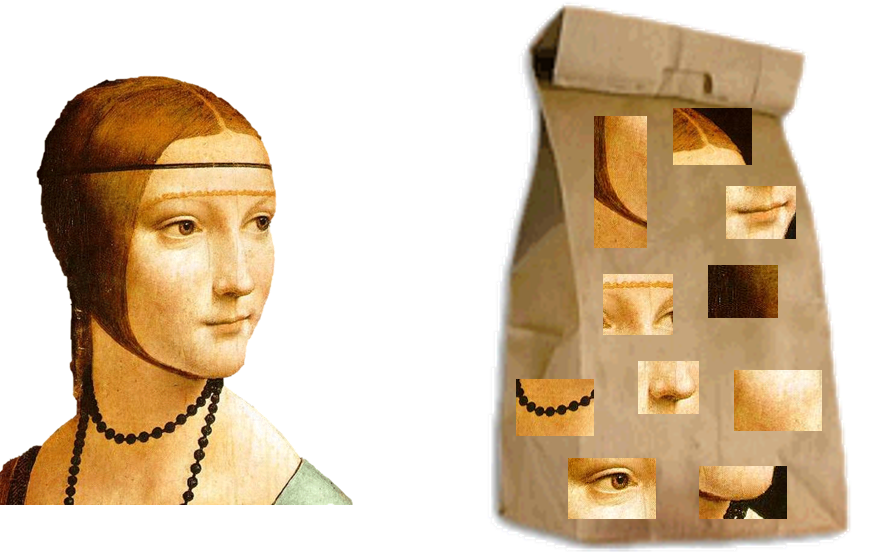
\includegraphics[width=\textwidth]{bow.png}
\caption{BOW模型}
\end{figure}

词袋模型在图像上提取局部特征点,并通过kmeans等方法将特征向量聚类,形成视觉单词的码书。在线检索时,通过将提取到的局部特征点映射为视觉单词,则可以将整个图像看做是由视觉单词组成的文本,从而可以应用文本检索的经典方法来对图像进行检索。下面我们将对基于BOF模型的图像检索系统进行简单的介绍。


\subsection{SIFT特征提取}
SIFT,即尺度不变性特征(Scale-invariant feature transform, SIFT),是图像处理与计算机视觉领域广泛使用的一种局部特征描述子\cite{lowe2004distinctive}。其具有以下一些特性:
\begin{enumerate}
\item SIFT特征是图像的局部特征,对旋转、尺度缩放、亮度变化等均具有不变形,对视角变化、仿射变换、噪声也具有一定程度的稳定性;
\item 独特性好,信息量丰富,适于在海量特征数据库中进行快速、准确的匹配;
\item 多量性,即使少数的几个物体也可以产生大量的SIFT特征向量;
\item 高速型,经优化的SIFT匹配算法甚至可以达到实时的要求;
\item 可扩展性,可以很方便的与其他形式的特征向量进行联合;
\end{enumerate}
正是因为SIFT具有以上特性,BOF模型通常都选用SIFT对图像局部特征进行描述。SIFT特征检测主要包括以下4个基本步骤:
\begin{enumerate}
\item 尺度空间极值检测:搜索所有尺度上的图像位置,通过高斯微分函数来识别潜在的对于尺度和旋转具有不变性的兴趣点。
\item 关键点定位:在每个候选位置上,通过一个拟合精细的模型来确定位置和尺度,依据候选点的稳定程度选取关键点。
\item 方向确定: 基于图像局部的梯度方向,分配给每个关键点位置一个或多个方向,后面对关键点的特征描述都相对于关键点的方向,尺度和位置进行变化,从而保证特征描述的不变性。
\item 关键点描述:在每个关键点周围的领域内,根据所选尺度,在图像局部计算梯度直方图,并连接为一个128维的向量。
\end{enumerate}

\subsection{建立码书}
对于每个图像提取得到若干的SIFT特征点向量,然后对所有图像的特征向量进行聚类,通常使用kmeans聚类,最后将聚类得到的聚类中心作为视觉单词,形成码书。假设要形成k个视觉单词,kmeans算法描述如下:
\begin{enumerate}
\item 适当选择k个类的初始中心;
\item 在第i次迭代中,对任意一个样本,求其到k个中心的距离,将该样本归到距离最短的中心所在的类;
\item 利用均值等方法更新该类的中心值;
\item 对于所有的k个聚类中心,如果重复利用2,3步骤进行迭代更新后,值保持不变(或者指定一个变化阈值),则迭代结束,否则继续迭代。
\end{enumerate}
在实际操作中,通常在另外一个数据集上提取特征并建立码书,视觉单词数量k通常选取20k至200k之间。

\subsection{倒排索引}
在线实际检索时,由于通常图像库很大(例如百万级别),此时如果通过线性比较计算图像之间的相似性,速度是不可忍受的,为此需要建立某种形式的索引,以提高检索效率。通常采用倒排索引。
\begin{figure}[h]
\centering
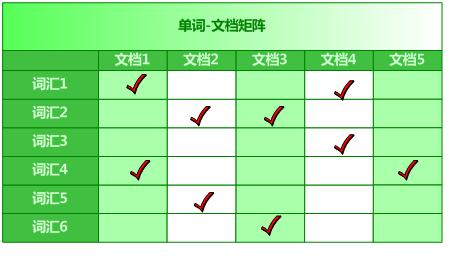
\includegraphics[width=\textwidth]{invindex.jpg}
\caption{倒排索引示例}\label{fig:invindex}
\end{figure}
如图\ref{fig:invindex}所示为一个单词-文档矩阵,其中打勾则代表包含关系。从纵向即文档的维度来看,每列代表文档包含了哪些单词,即正向索引。而横向即从单词的维度来看,每行代表了哪些文档包含了某个单词。倒排索引即从单词的维度来看,建立的单词-文档矩阵。如此建立索引后,每次在线查询时,只需要将得到的局部特征映射为视觉单词,然后通过倒排索引的单词-文档矩阵,就可以查找到所有包含该单词的文档,最后通过tf-idf进行评分,即可将相关的文档进行评分。倒排索引高效的关键在于,每个文档包含的视觉单词只是整个码书很小的一部分,即单词-文档矩阵是稀疏的,这样在检索时,只需要计算码书中非0部分的评分,从而避免了在整个码书上计算。

\subsection{整体系统框架}
\begin{figure}[h]
\centering
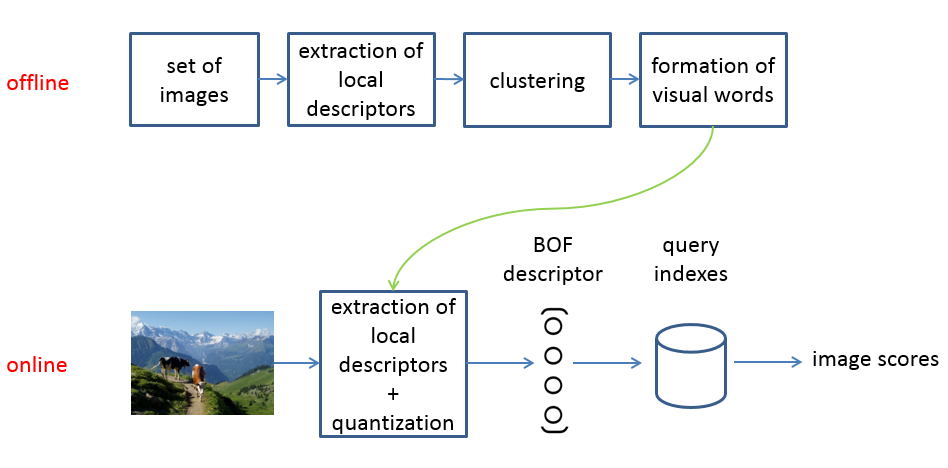
\includegraphics[width=\textwidth]{bowframework.png}
\caption{BOW模型框架图}\label{fig:bowframework}
\end{figure}
整体框架如图\ref{fig:bowframework}所示,离线训练时,我们从一组图像集合中提取局部特征,然后对其进行kmeans聚类,我们将聚类中心作为视觉单词,形成码书。在线检索时,我们首先提取图像的局部点特征(SIFT),然后将每一个点特征进行量化(查找与码书中的视觉单词欧氏距离最近的单词),形成词频向量,最后通过倒排索引,对相关图像进行评分,排序后,输出相关文档(图像)。

\section{利用显著区域检测优化结果}
\subsection{问题来源}
\begin{figure}[h]
\centering
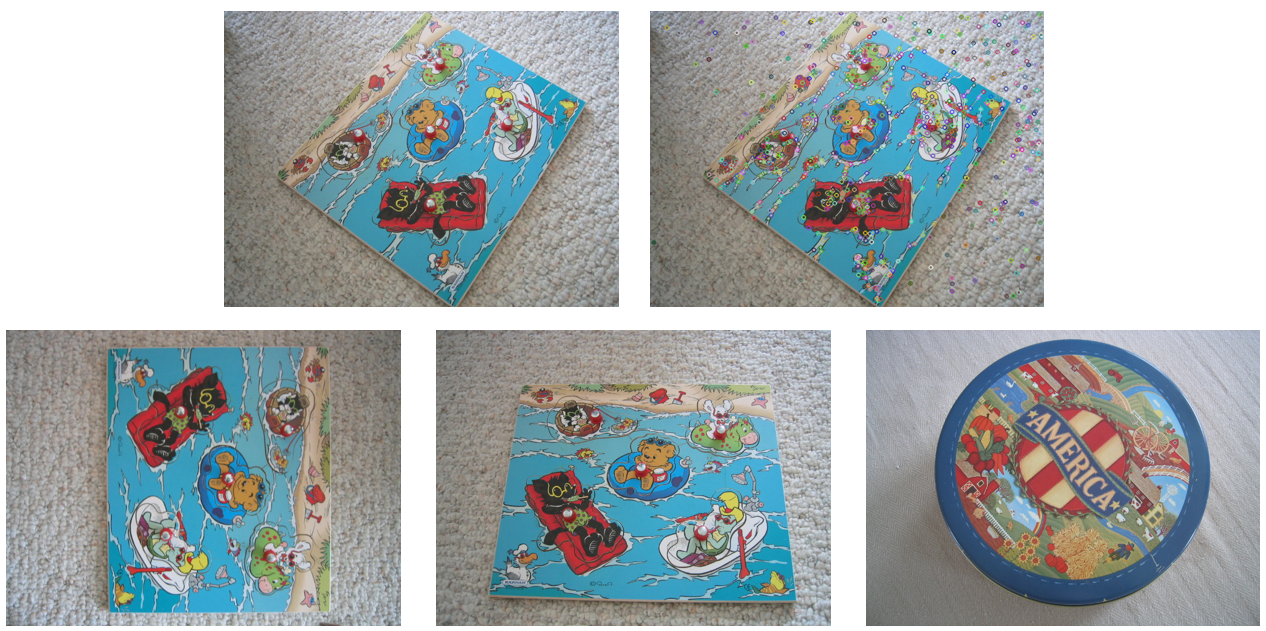
\includegraphics[width=\textwidth]{problem.png}
\caption{检索示例}\label{fig:problem}
\end{figure}
如图\ref{fig:problem}所示,第一行左边的图像为输入图像,第二行为检索结果的前三幅图像,可以看到第三幅图像是错误的。第一行右边的图像上表示了检测到的SIFT关键点,可以看到,在该图像的背景上也提取到了很多SIFT点,这些SIFT点与第三幅图像背景上的点匹配上了,因而影响了检索的精度。

可以看到,背景元素通常与用户的检索意图无关,然而背景元素上提取到的特征点,却同样参与了图像相关性的评分,因而会影响到检索的精度。

\subsection{优化方案}
我们采用显著区域检测做预处理,将前景和背景分离出来,提取特征点的时候,只在显著区域计算特征点,而忽略背景区域的特征点。这样做的好处有两个:
\begin{enumerate}
\item 剔除了背景上的特征点,提高检索精度,使得检索结果更加贴合用户意图。
\item 提升了检索速度。首先特征提取只需在显著区域进行计算,其次,得到更少的特征后,需要在倒排索引上检索的次数同时也减少了。
\end{enumerate}
在实验中,我们选取了前一章中介绍的基于蒙特卡洛采样的显著区域检测算法。

\section{实验结果}
\subsection{数据集和评价指标}
我们使用了ukbench数据集\cite{nister2006scalable},这个数据集包含2550种不同的物体或场景,每一个物体(场景)都包含4幅从不同角度拍摄的图像,整个数据集一共有10200幅图像。对于这个数据集,我们采用两种评价指标:mAp(mean Average Precision)和KS(Kentucky Score),KS指标是该数据集的作者针对该数据集提出的评价指标,即取top 4的结果中,正确结果的平均值。另外,为了更加客观的比较优化方案的优化效果,我们分别取码书大小为10k和100k的结果做比较。
\subsection{实验结果}
\begin{table}
\centering
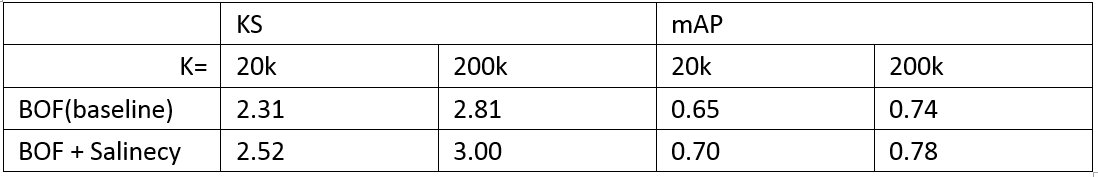
\includegraphics[width=\textwidth]{exp.png}
\caption{实验结果}
\end{table}
如表所示,可以看到,在添加了显著区域检测进行特征点的过滤后,KS值提高了0.2左右,同时mAp提高了5个百分点左右,实验证明,显著区域检测对图像检索确实有一定的提升作用。
